%!TEX program = lualatex
\documentclass[25pt]{tikzposter}
\usepackage[spanish]{babel}
\usetheme{Envelope}
\usebackgroundstyle{Rays}
\usenotestyle{VerticalShading}
\usepackage[math]{kurier}
\geometry{paperwidth=100cm, paperheight=130cm}
\makeatletter
\setlength{\TP@visibletextwidth}{\textwidth-2\TP@innermargin}
\setlength{\TP@visibletextheight}{\textheight-2\TP@innermargin}
\makeatother

\title{\parbox{\linewidth}{\centering Smart Usage of Context Information for the Analysis, Design, and Generation of Power-Aware Policies for Mobile Sensing Apps}}
\author{Rafael Pérez Torres, Dr. César Torres Huitzil, Hiram Galeana Zapién Phd}
\institute{LTI Cinvestav Tamaulipas}
\titlegraphic{
\includegraphics[scale=0.8]{./images/cinvestav-logo-no-text-white}}

\makeatletter
\renewcommand\TP@maketitle{%
   \centering
   \begin{minipage}[b]{0.7\linewidth}
        \centering
        \color{titlefgcolor}
        {\bfseries \Huge \sc \@title \par}
        \vspace*{1em}
        {\huge \@author \par}
        \vspace*{1em}
        {\LARGE \@institute}
    \end{minipage}%
    \tikz[remember picture,overlay]\node[scale=0.8,anchor=east,xshift=-45cm,yshift=6cm,inner sep=0pt] {%
       \@titlegraphic
    };
}
\makeatother

\begin{document}
\maketitle
\block{Resumen}{
	\Large
	Los servicios móviles basados en localización ejecutados por smartphones requieren actualizaciones constantes de ubicación para adaptar su funcionamiento.
	Sin embargo, realizar el seguimiento del usuario mediante proveedores de ubicación clásicos, como el GPS, representa un alto consumo de energía, la cual es un recurso escaso y competido en este tipo de platformas.
	La presente investigación tiene como objetivo reducir el consumo de energía al realizar el seguimiento del usuario, a partir de información contextual que es extraída de datos provenientes de los sensores.
	Dicha información permite al dispositivo aprender sobre los patrones de movilidad del usuario y apoyarse en este conocimiento para realizar un uso adaptativo de los proveedores de ubicación.
}

\begin{columns}
	\column{0.5}
	\block{Antecedentes}{
		% \Large
		\begin{itemize}
		  \item La energía es un recurso limitado en plataformas móviles, como el smartphone.
		  \item Por ello, el sensado constante (o indiscriminado) no resulta óptimo, descargando rápidamente la batería.
		  \item Es posible explorar estrategias alternativas para realizar el monitoreo continuo del usuario, atendiendo al compromiso energía-precisión.
		  \item Tal es el caso del uso de información contextual, la cual permite caracterizar la situación del usuario y emplearla para adaptar de forma dinámica el acceso al GPS.
		\end{itemize}
	}

	\column{0.5}
	\block{Problema}{
		% \Large
		\begin{enumerate}
			\item Utilizar datos de los sensores para identificar y aprender acerca de la actividad del usuario así como su ubicación $\rightarrow$ \textbf{identificar y aprender patrones de movilidad}.
			\item Utilizar la información aprendida para mejorar el uso de los proveedores de ubicación (GPS) del dispositivo, considerando el compromiso entre \emph{precisión - consumo de energía}. $\rightarrow$ \textbf{Producir políticas conscientes de la energía}.
		\end{enumerate}
	}
\end{columns}

\begin{columns}
\column{0.5}
\block{Fundamentos de la solución propuesta}{
	\begin{tikzfigure}[Componentes de un sistema dirigido por eventos]
		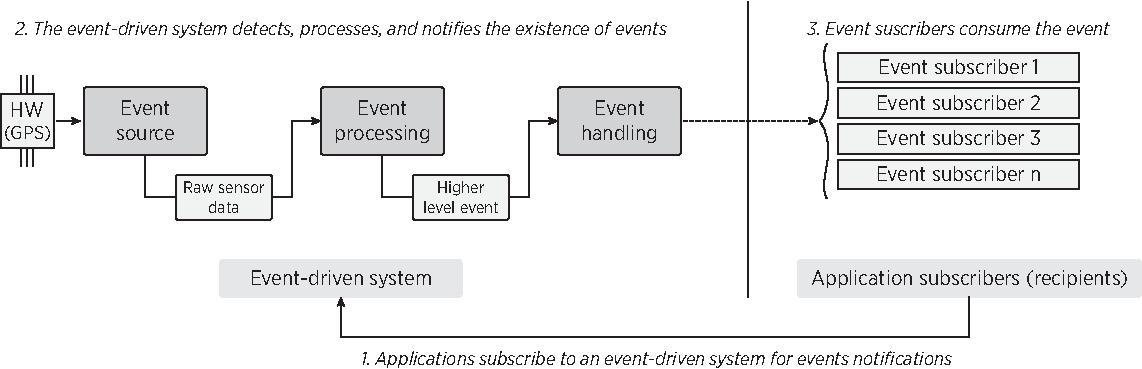
\includegraphics[width=0.32\textwidth]{images/event-driven-system.pdf}
	\end{tikzfigure} 
	\begin{tikzfigure}[Variaciones de la velocidad de acuerdo a los patrones de movilidad]
		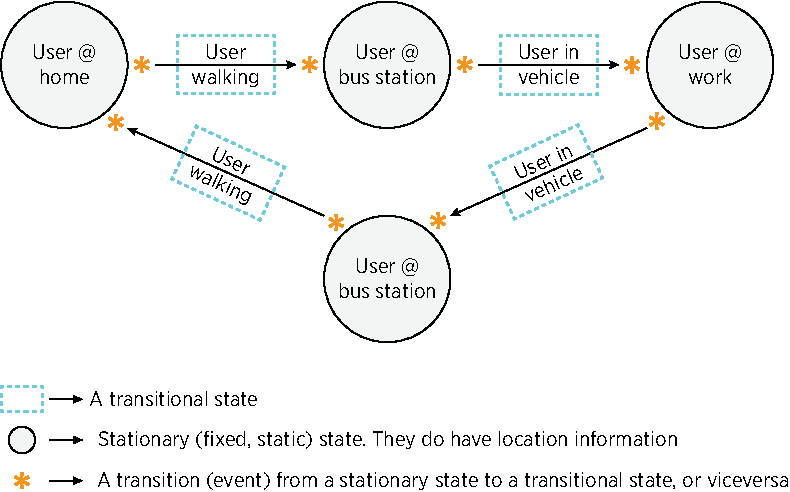
\includegraphics[width=0.27\textwidth]{images/physics-perspective-of-motion}
	\end{tikzfigure}
	\begin{tikzfigure}[Estructura de un sistema cognitivo dinámico]
		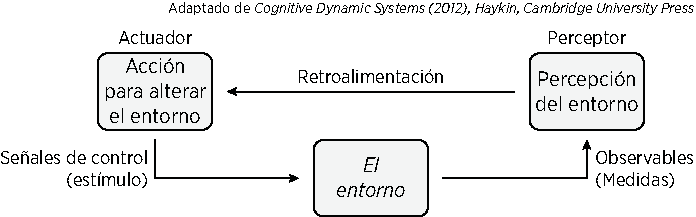
\includegraphics[width=0.21\textwidth]{images/cognitive-dynamic-systems.pdf}
	\end{tikzfigure}  
}

% \block{Sistemas dirigidos por eventos (Event-Driven Systems)}{
% 	\begin{tikzfigure}[Componentes de un sistema dirigido por eventos]
% 		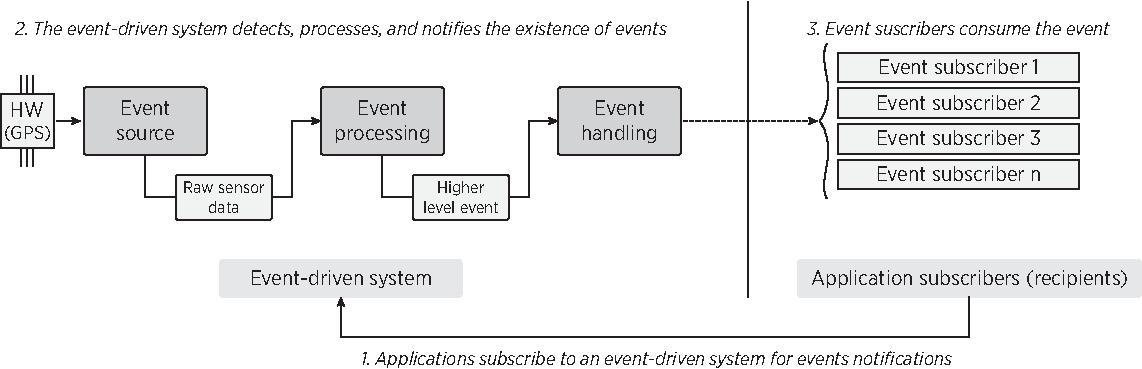
\includegraphics[width=0.32\textwidth]{images/event-driven-system.pdf}
% 	\end{tikzfigure} 
% }

% \block{Movimiento desde la perspectiva de la física}{
% 	\begin{tikzfigure}[Variaciones de la velocidad de acuerdo a los patrones de movilidad]
% 		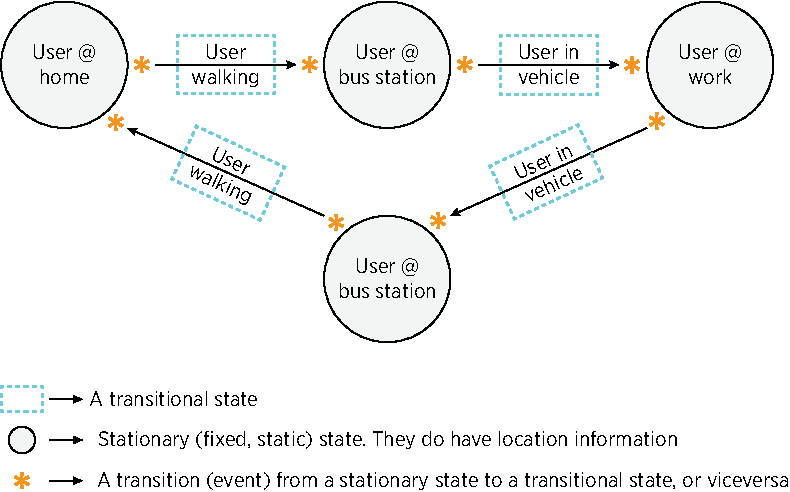
\includegraphics[width=0.27\textwidth]{images/physics-perspective-of-motion}
% 	\end{tikzfigure}
% }

% \block{Sistemas cognitivos dinámicos}{
% 	\begin{tikzfigure}[Estructura de un sistema cognitivo dinámico]
% 		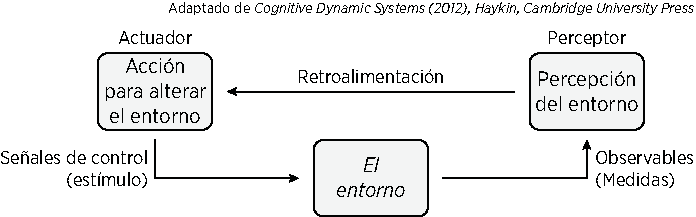
\includegraphics[width=0.21\textwidth]{images/cognitive-dynamic-systems.pdf}
% 	\end{tikzfigure}  
% }

\column{0.5}
\block{Solución Propuesta}{
	\begin{tikzfigure}[Arquitectura de la solución propuesta]
		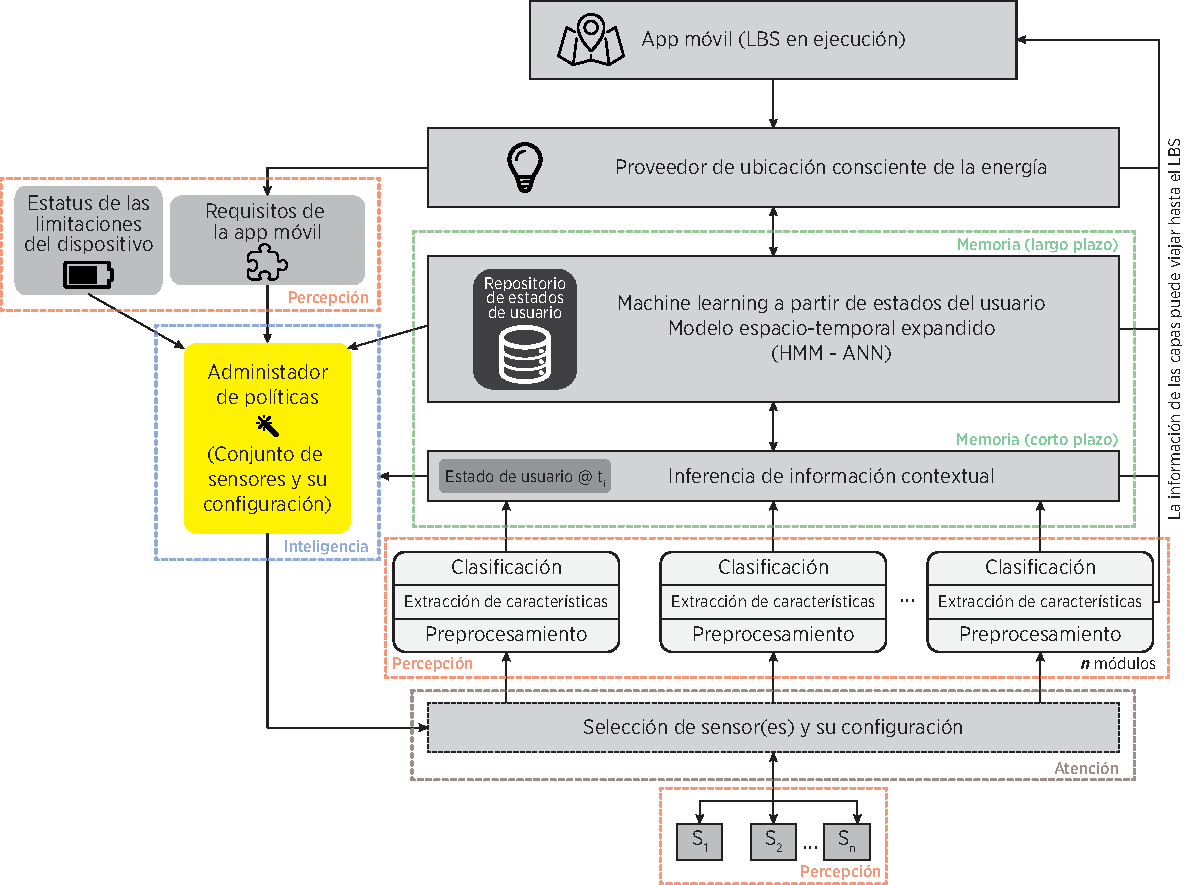
\includegraphics[width=0.35\textwidth]{images/solution-general-overview.pdf}
	\end{tikzfigure}
	\hfill
	\begin{tikzfigure}[Modelo espacio-temporal expandido de la solución propuesta]
		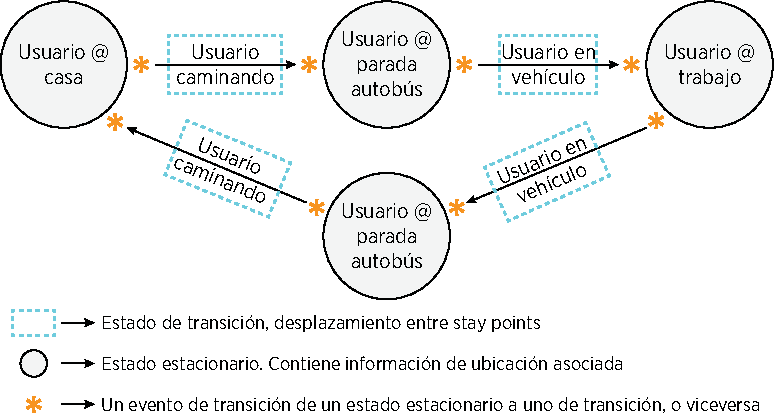
\includegraphics[width=0.24\textwidth]{images/zoom-expanded-spatial-time-model.pdf}
	\end{tikzfigure}
}
\end{columns}

\block{Resultados preliminares}{
	\begin{center}
		\begin{minipage}{0.65\linewidth}
	  		\centering   
	    	\begin{tikzfigure}[Stay points obtenidos de forma autónoma por el smartphone]
		    	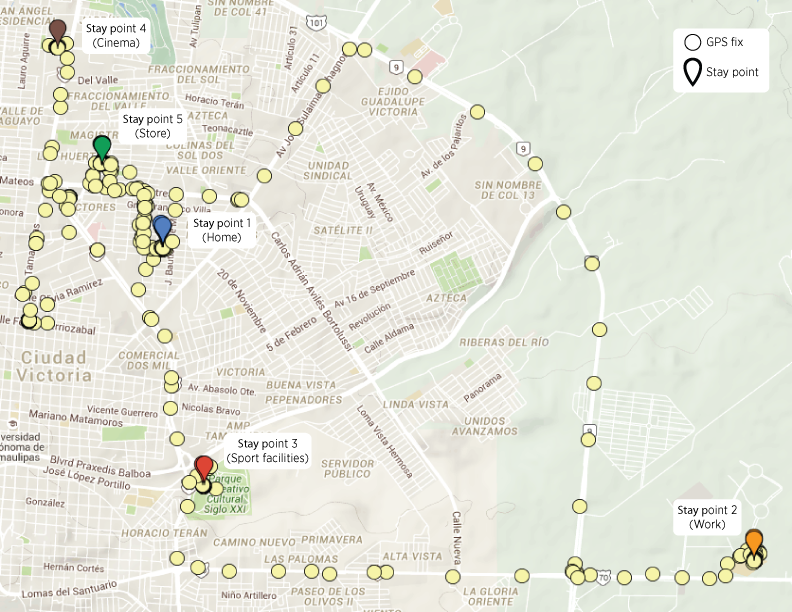
\includegraphics[width=0.34\textwidth]{images/map}
		    	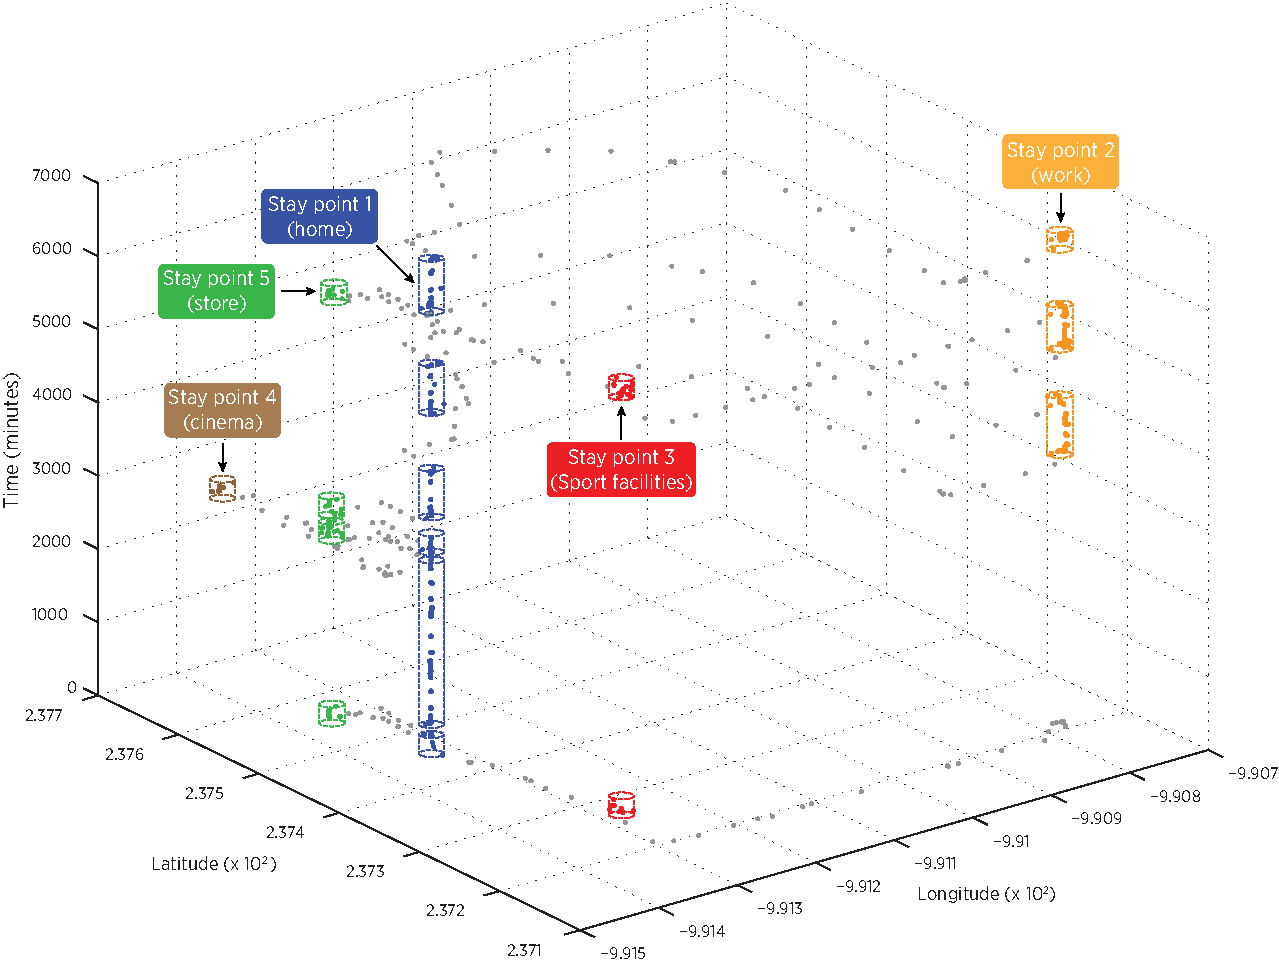
\includegraphics[width=0.34\textwidth]{images/map-three-dimensional}
	    	\end{tikzfigure}
    	\end{minipage}~~~\hfill
		\begin{minipage}{0.35\linewidth}
			\centering
			\begin{tikzfigure}[Módulo HAR capaz de detectar la actividad física del usuario]
    			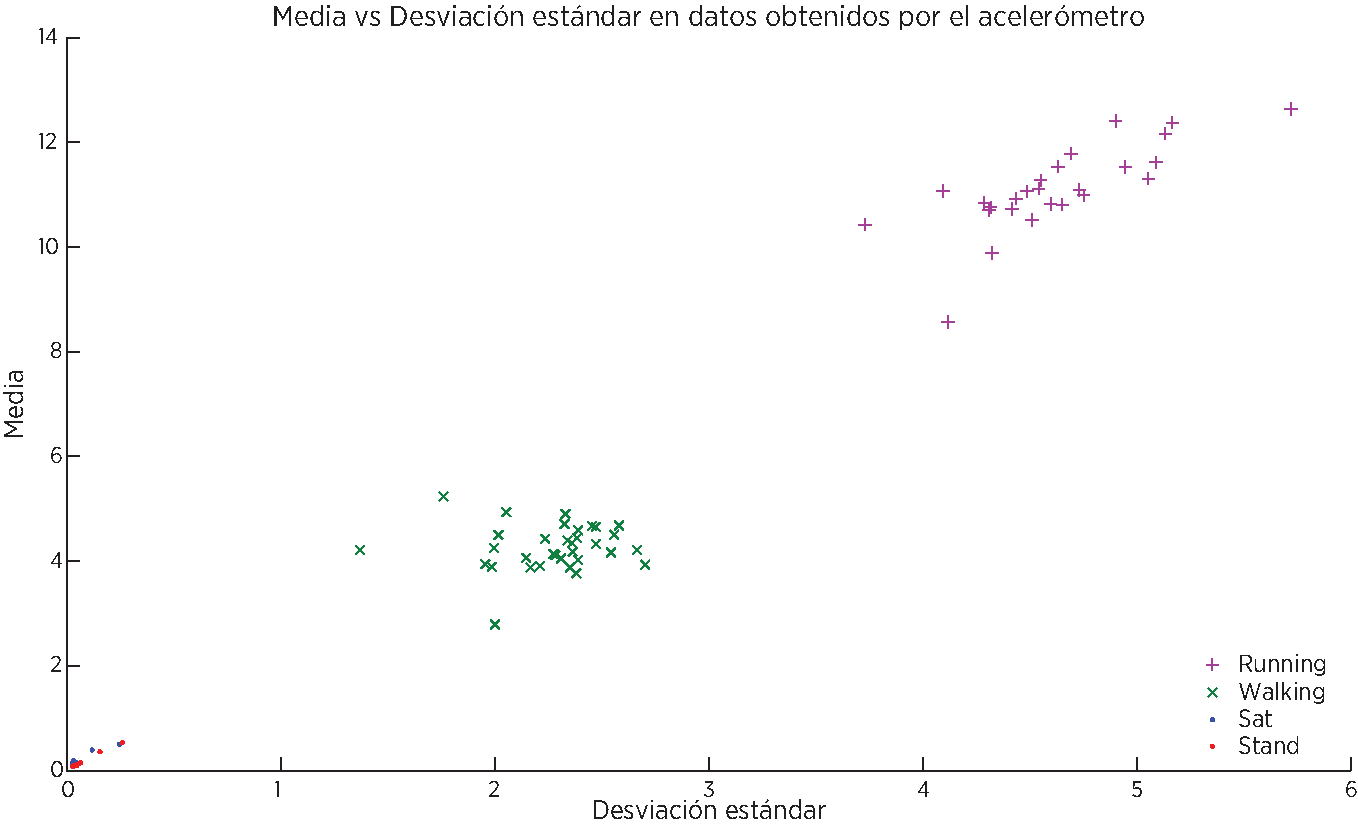
\includegraphics[width=0.8\textwidth]{images/plot-mean-sd.pdf}
			\end{tikzfigure}
		\end{minipage}
	\end{center}
}

\end{document}